\documentclass[a4paper]{article}
\usepackage[utf8]{inputenc}
\usepackage{fancyhdr}
\usepackage{vmargin}
\usepackage{listings}

%nicer tables
\usepackage{booktabs}

\usepackage{graphicx}

\usepackage{float}

\usepackage{color}
\usepackage{url}
\usepackage{hyperref}

\usepackage{enumerate}

\usepackage[backend=biber]{biblatex}

\usepackage{csquotes}

\usepackage{multicol}
\setlength{\columnsep}{1cm}
\setlength{\headheight}{36pt}

\definecolor{bluekeywords}{rgb}{0.13,0.13,1}
\definecolor{greencomments}{rgb}{0,0.5,0}
\definecolor{redstrings}{rgb}{0.9,0,0}



%
\usepackage{amsmath, amsthm, amssymb}
\usepackage[ngerman, english]{babel}
\usepackage{marvosym}
\usepackage{graphics}
\usepackage{extarrows}
\usepackage{forloop}
\usepackage{mathtools}

\usepackage[]{algorithm2e}

\usepackage{hyperref}% http://ctan.org/pkg/hyperref
\usepackage{cleveref}% http://ctan.org/pkg/cleveref
\usepackage{lipsum}% http://ctan.org/pkg/lipsum
\newtheorem{definition}{Definition}
\newtheorem{theorem}{Theorem}
\newtheorem{lemma}{Lemma}
\newtheorem{preliminary}{Preliminary}
\newtheorem{notation}{Notation}
\newtheorem{property}{Property}
\newtheorem{corollary}{Corollary}
\newtheorem{example}{Example}
\newtheorem{hypothesis}{Hypothesis}

\crefname{theorem}{Theorem}{Theorems}
\crefname{definition}{Definition}{Definitions}
\crefname{lemma}{Lemma}{Lemmas}
\crefname{preliminary}{Preliminary}{Preliminaries}
\crefname{notation}{Notation}{Notations}
\crefname{property}{Property}{Properties}
\crefname{corollary}{Corollary}{Corollaries}
\crefname{example}{Example}{Examples}
\crefname{hypothesis}{Hypothesis}{Hypotheses}

\newenvironment{beweis}{\begin{proof}[Beweis]}{\end{proof}}
%



\lstset{language=Python,
showspaces=false,
showtabs=false,
breaklines=true,
showstringspaces=false,
breakatwhitespace=true,
escapeinside={(*@}{@*)},
commentstyle=\color{greencomments},
keywordstyle=\color{bluekeywords}\bfseries,
stringstyle=\color{redstrings},
basicstyle=\ttfamily
}


\setlength{\parindent}{0pt}
\setlength{\parskip}{5pt}

\frenchspacing
\pagestyle{fancy}
\sloppy 

\markright{headline}

\addbibresource{references.bib}

\begin{document}

\lhead{\begin{tabular}{l}
\\
Neural Networks\\
WiSe 2020/2021\\
\end{tabular}}

\rhead{\begin{tabular}{r}
Assignment 8\\
Simon Laurent Lebailly, 2549365, s9sileba@teams.uni-saarland.de\\%% <=== Also HERE if you have a team mateUpdate Name HERE !!! 
Christian Mathieu Schmidt, 2537621, s9cmscmi@teams.uni-saarland.de
\end{tabular}}




\section*{Exercise 8.1: Empirical Risk Minimization}
    \subsection*{a)}
        As expected risk we denote the expected generalization error, which is the expected value taken over the true underlying unknown distribution $p_{data}(x,y)$ of data:
        When we replace the true distribution $p_{data}(x,y)$ by the empirical distribution $\hat{p}_{data}(x,y)$ defined by the training set, we convert the initial problem from a machine learning problem to an optimization problem.
        So we do not optimize the expected risk, but the empirical risk:
        \begin{align}
            \mathbb{E}_{x,y \sim \hat{p}_{data}(x,y)}[L(f(x;\theta),y)] = \frac{1}{m} \sum\limits_{i=1}^m L(f(x^{(i)};\theta),y^{(i)})
        \end{align}
        where $m$ is the number of training examples, and $\theta$ are the parameters.\\
        The sense is that we do not optimize the true risk directly, but the empirical risk instead.
        Through this optimization, the true risk should also be minimized!\\
        (Source of inspiration: Deep Learning book by Ian Goodfellow, page 272,273)


    \subsection*{b)}
        

    
    \subsection*{c)}
        \begin{itemize}
            \item ERM is a problem with very high computational complexity.
            Even for simple functions and simple classes it is an NP-hard problem.
            \item ERM has the problam, that the result depends from the derivative of the function.
            But there are a lot functions which do not have useful derivatives.
            For example, the derivative of a linear function is a constant, and thats not very useful!
        \end{itemize}




\newpage
\section*{Exercise 8.2: First-Order Optimization}
    \subsection*{a)}
        \begin{center}
            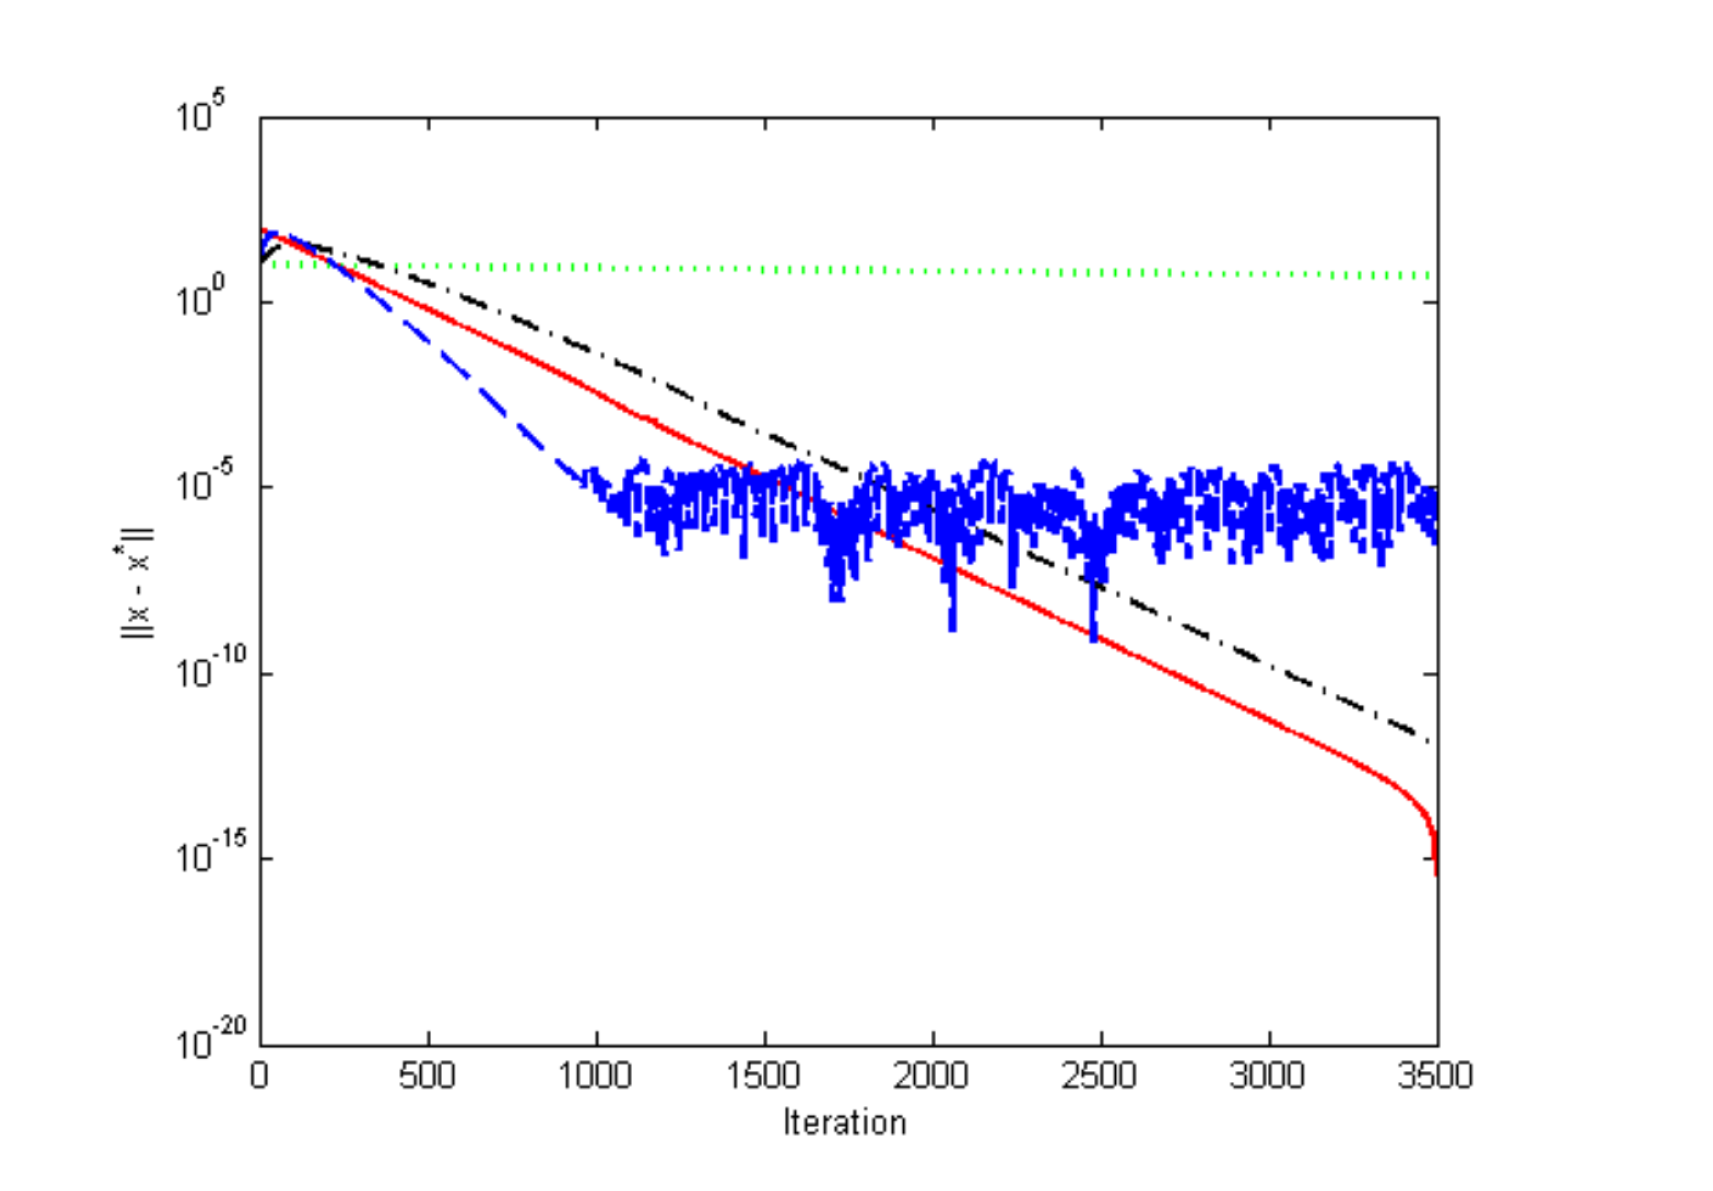
\includegraphics[width=120mm]{Assignment 8/A8_3_a.png}
        \end{center}
        \begin{itemize}
            \item \textbf{Method 1: BLUE line}\\
                Because of the constant step-size and the general behavior of such a method, we can see that the blue line corresponds to the gradient method.
                At the beginning, the method approaches the minimum very quickly, i.e. with only a few iterations (ca. 1000). 
                But because of the constant step-size and the general behavior of a gradient method, it always jumps back and forth between the slopes of the function, missing the minimum every time, and therefore not minimizing the loss any further.
            
            \item \textbf{Method 2: GREEN line}\\
                Method 3 corresponds to the green line, because $\lim\limits_{k \rightarrow \infty} (1-2\sqrt{\frac{m}{L}})^kC = 0$ for a constant $C$ with $k$ as the number of iterations.
                So $f(x_k) - f(x^*)$ which is always less equal the above expression, falls in the same velocity, and therefore the loss converges against zero, which is illustrated by the green line.
            
            \item \textbf{Method 3: BLACK line}\\
                
            
            \item \textbf{Method 4: RED line}\\
                NAG evaluate the gradient after the current velocity is applied.
                Therefore it add a correction factor to the standard method of momentum and decreases the excess error from $\mathcal{O}(\frac{1}{k})$ (after $k$ steps) to $\mathcal{O}(\frac{1}{k^2})$ in the convex gradient batch.
                This advantage we can see if we consider the black line (Method 3) and the red line.
                Just before 3500 iterations, we can see that the red line starts to fall much harder as the black line.
                But it falls all the time faster than the black line, and we can see that the red line is falling faster and faster in relation to the black line.
                
            
        \end{itemize}

    
    \subsection*{b)}
        


    \subsection*{c)}
        



\newpage
\section*{Exercise 8.3: Second-Order Optimization}
    \subsection*{a)}
        First-Order optimization methods only look for the gradient to find the local minimum.
        Second-Order optimization methods also find a downhill direction, but they consider not only the gradient, they also consider the curvature.
        Thus, if the algorithm comes closer to a local maximum, the Hessian will be positive definite.
        If the algorithm comes closer to a local minimum, the Hessian will be negative definite.
        And if the algorithm comes closer to a saddle point, the Hessian will have positive and negative eigenvalues.\\
        In short, unlike first-order optimization methods, second-order optimization methods do not ignore the curvature of a surface and thus improve the result in each individual optimization step.\\
        
        Since we derive twice it is of course necessary that the function is twice differentiable.
        

    \subsection*{b)}
        Definition of Taylor series and Newton's method from Deep Learning book by Ian Goodfellow (page 307).
        Approximation of $J(\theta)$ near some point $\theta_0$ with second-order Taylor series, ignoring derivatives of higher order:
        \begin{align}
            J(\theta) &\approx J(\theta_0) + (\theta - \theta_0)^T \nabla_{\theta} J(\theta_0) + \frac{1}{2} (\theta - \theta_0)^T H(\theta - \theta_0)
        \end{align}
        where $H$ is the Hessian of $J$ with respect to $\theta$ evaluated at $\theta_0$.\\
        The Newton parameter update rule:
        \begin{align}
            \theta^* &= \theta_0 - H^{-1} \nabla_{\theta} J(\theta_0)
        \end{align}
        \textbf{Usability of Newton Method:}\\
        With the Newton method one tries to approach the minimum of a function by approaching the zero of the derivative, which belongs to this minimum.
        Thereby the distance of the zero point of the tangent of the derivative at the momentarily considered point is approached more and more to the zero point of the derivative.
        This intersection is then considered as a new point, which is why the Newton method is an iterative method.
        The distance of the intersection point of the tangent of the derivative at the momentarily considered point to the zero of the derivative decreases thereby quadratically.
        Thus Newton's method allows a fast approach to the zero of the first derivative by considering the first and second derivative.

    
    \subsection*{c)}
        The main difference is that quasi-Newton algorithms save computational effort by approximating the inverse of the Hessian matrix rather than computing it directly.
        Hereby the computational effort per iteration can be strongly reduced.
        The advantage of the normal Newton method is that fewer iteration steps are needed than with the gradient method, but disadvantageously the iteration steps themselves are much more expensive.
        The quasi-Newton algorithms are a compromise.
        The accuracy decreases, whereby one needs more iteration steps altogether, but the individual iteration steps can be accelerated by approximation of the inverse Hessian matrix.\\
        (Source of most of the information: Deep Learning book by Ian Goodfellow, page 312)

\newpage
    \subsection*{d)}
        BFGS attempts to approximate the inverse Hessian matrix iteratively.
        Here, the approximated matrix $M$ is iteratively refined by low-rank updates.
        Assuming we are in the $i$-th iteration, the $i+1$-th iteration is calculated as follows:\\
        When the matrix $M_i$ has been updated, the direction of descent $p_i$ is determined by $p_i = M_i g_i$.
        The stepsize $\epsilon^*$ is then updated by a line search through $g_i$ in the direction of $p_i$. This results in the following parameter update which does not depend on the inverse Hessian matrix $H^{-1}$:
        \begin{align}
            \theta_{i+1} &= \theta_i + \epsilon^* p_i
        \end{align}
        (Source of most of the information: Deep Learning book by Ian Goodfellow, page 312)


\end{document}
